
\section{Beskrivelse af de elektriske komponenter anvendt i kredsløbet}

Følgende er en kort teoretisk beskrivelse af, hvorledes de forskellige komponenter, som er anvendt i det elektriske kredsløb til blyantspidseren, virker. Dette giver et overblik over, hvilke egenskaber og funktioner de enkelte komponenter bidrager med, når kredsløbet senere bliver beskrevet som en helhed. 

  
\subsection{Komparator - generelt om operationsforstærkere}

Operationsforstærkeren har et inverterende og et ikke-inverterende input. 
Ideelt set er operationsforstærkeren kendetegnet ved, at den har uendelige inputsimpedanser, forstærkningen er uendelig, og der er ingen udgangsimpedans. Der anvendes ofte negativ eller positiv feedback ved operationsforstærkere. Det betyder, at dele af signalet bliver sendt fra output og tilbage til det inverternde input ved negativt feedback, mens det ved positivt feedback sendes til den ikke-inverterende input.  Hvis man anvender en operationsforstærker uden feedback, får man en komparator. Komparatoren er et element, som tager to strømme eller spændinger og sammenligner dem. Operationsforstærkeren kigger på det inverterende input i forhold til det ikke-inverterende input. Hvis det ikke inverterende input er større end det inverterende input vil den forstærke outputtet så meget den kan, mens hvis det inverterende input er større end det ikke-inverterende input, vil outputtet gå ned til den negative grænse. Den maksimale forstærkning bestemmes af operationsforstærkerens spændingskilde (eks. $\pm$ 15V).

\subsection{LED}
\begin{figure}[h]
	\begin{center}
	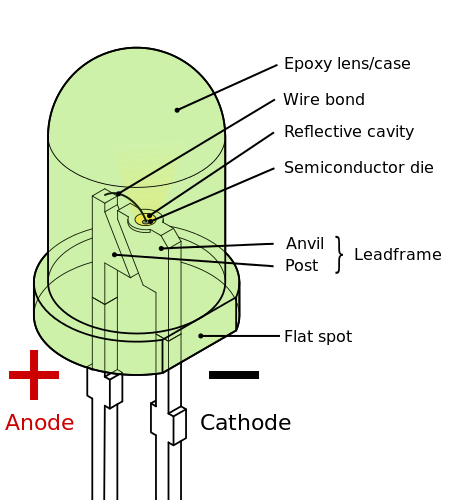
\includegraphics[scale=0.4]{Billeder/LED_Wiki.png}
	\caption[caption]{Oversigt over en LED (Light Emitting Diode)\label{fig:LED}\\\hspace{\textwidth}}
	\end{center}
\end{figure}
Dioden har to terminaler (som ses på figur ~\ref{fig:LED}), anoden og katoden. Hvis man sætter en lille, positiv spænding til en diode vil den få en høj strøm. Dette kaldes forward bias. Hvis der på den anden side er en negativ spænding, skal denne være noget større for at få en strøm til at løbe. Dette kaldes reverse-bias. Dette anvendes til at lade en strøm løbe den ene vej gennem en diode, men blokere for strømmen i modsat retning. Dioder består af et knudepunkt mellem halvledermateriale. På den ene side af knudepunktet dannes n-materiale, hvor der er et stort overskud af frie elektroner, mens der på den anden side dannes p-materiale, hvor der er overskud af "huller". Dette betyder, at selvom man ikke sætter nogen strøm til, vil der stadig være et elektrisk felt, som holder de frie elektroner på n-siden og hullerne på p-siden. Hvis en ydre positiv spænding sættes på n-siden, kan ladningsbærerne ikke krydse knudepunktet, og der går ingen strøm. Hvis der derimod sættes en positiv spænding på p-siden, bliver feltet mindre, og der vil derfor kunne gå en strøm.  
En LED, som er en light emitting diode, er således en diode, som lyser, når den aktiveres. Dette sker, når en elektron flyttes til et hul, udgiver den energi i form af en foton. 


\subsection{MOSFET}

Transistorer anvendes i al elektronik, hvor hukommelse anvendes. Den mest anvendte transistor er MOSFET’en, som er en af to transistorer, der bliver anvendt i kredsløbet til styring af blyantspidseren. 
Til forskel fra en almindelig npn transistor, der er strømstyret, er MOSFET’en spændingstyret. Fordelen ved en MOSFET er, at den ikke kræver en særlig stor strøm (tæt på ingen) ind i gaten for at aktivere den, men den kan stadig (for nogle typer) levere op til 50 ampere eller mere til et load. Størrelsen af strømmen, den kan håndtere, afhænger af hvordan MOSFET’en er bygget, og dens fysiske størrelse.

\begin{figure}[h]
	\begin{center}
	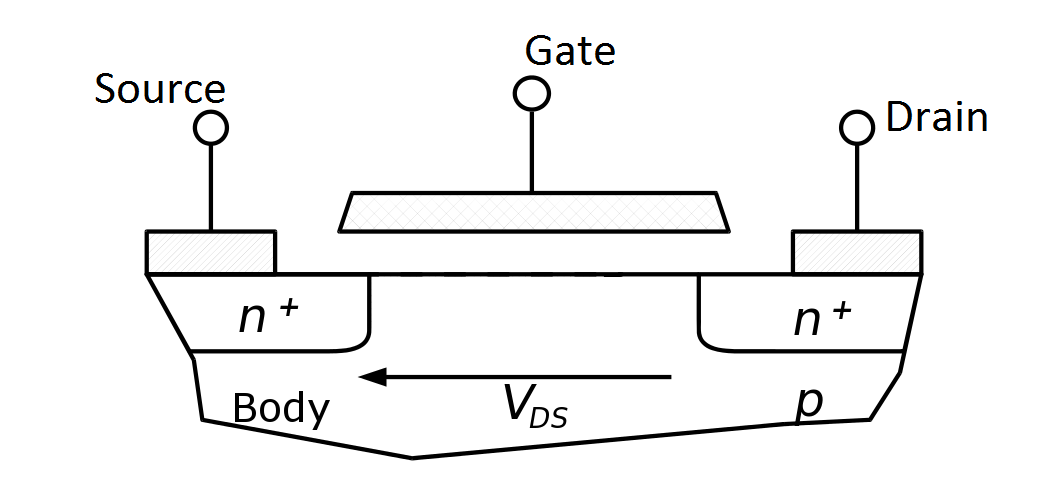
\includegraphics[scale=0.15]{Billeder/MOSFET.png}
	\caption[caption]{Oversigt over en MOSFET (Metal-Oxide-Semiconductor Field-Effect Transistor)\label{fig:MOSFET}\\\hspace{\textwidth}}
	\end{center}
\end{figure}
 
MOSFET’en har fire terminaler (som ses på figur ~\ref{fig:MOSFET}); source, drain, gate og body. Der bliver dog ofte kun refereret til de tre førstnævnte, da source og body er ofte forbundet med hinanden, og dermed danner én terminal (kaldet source). I kredsløbet for blyantspidseren bruges en npn-type, og den anvendes som en switch, der fungerer ved, at den har et ON- og OFF-stadie. Om den er ON eller OFF afgøres af spændingsfaldet over gate- og sourceterminalen. Ved OFF-stadiet er der intet spændingsfald over gaten, hvilket forhindrer elektroner i at strømme fra drain til source, da der dannes et bånd af ioner, kaldet en depletion region, som reflekterer elektronerne kommende fra drain til source. Sættes der spænding over gaten, vil MOSFET’en tillade, at der løber en strøm ved at hjælpe en vis mængde elektroner gennem depletion regionen. Denne mængde afhænger af størrelsen på spændingen over gaten. Jo højere spænding desto større flow af elektroner. I kredsløbet for blyantspidseren er spændingen på gaten altid enten nul eller en bestemt værdi, der ikke varierer (styret af operationsforstærkeren), så den som nævnt kan fungere som en switch, der enten afbryder strømmen, eller lader den passere til blyantspidserens behov ved at simulere en kortslutning. Source er forbundet til ground og har derfor et potentiale på 0V.

\subsection{Fototransistor}

\begin{figure}[h]
	\begin{center}
	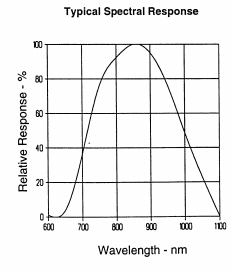
\includegraphics[scale=0.4]{Billeder/Fototransistor_respons.png}
	\caption[caption]{Diagram over fototransistorens respons på foskellige bølgelængder af lys\label{fig:OP598}\\\hspace{\textwidth}}
	\end{center}
\end{figure}
Fototransistoren fungerer stort set ligesom transistoren, som er beskrevet under afsnittet MOSFET. Dog har den ”almindelige” transistor tre andre terminaler end MOSFET’en: En base, en emitter og en collector. I modsætning til MOSFET’en, der behøver en spænding over sig for at starte strømflowet gennem transistoren, skal en fototransistor bruge lys for at åbne. Fototransistoren åbner gradvist op, afhængigt af hvilken bølgelængde den modtager - den kan eksempelvis åbne op for en hvis bølgelængde i det infrarøde spektrum. Forskellige bølgelængder har forskellige fordele ift. dens anvendelse. Vil man undgå, at fototransistoren bliver påvirket af almindeligt lys (ca. 400-700 nm), kan man eksempelvis vælge en, der åbner for infrarødt eller ultra violet lys. Graden, der bliver åbnet op med, afhænger af lysets indfaldsvinkel ift. sensoren, hvor kraftigt lyset er, og hvilke bølgelængder fototransistoren modtager. Kigger man f.eks. på figur ~\ref{fig:OP598}, har fototransistoren en respons mellem 40\% og 100\% i bølgelængderne, der svarer til infrarødt lys. Ved ca. 860 nm vil transistoren have en respons på 100\%, hvilket vil sige, at transistoren lader en maksimal mængde strøm passere.


